\documentclass[letterpaper,12pt]{article}

\usepackage{threeparttable}
\usepackage{geometry}
\geometry{letterpaper,tmargin=1in,bmargin=1in,lmargin=1.0in,rmargin=1.0in}
\usepackage[format=hang,font=normalsize,labelfont=bf]{caption}
\usepackage{amsmath}
\usepackage{multirow}
\usepackage{array}
\usepackage{delarray}
\usepackage{amssymb}
\usepackage{amsthm}
\usepackage{lscape}
\usepackage{natbib}
\usepackage{setspace}
\usepackage{float,color}
\usepackage[pdftex]{graphicx}
\usepackage{listings}
\lstset{basicstyle=\footnotesize\ttfamily, language=Python, showstringspaces=false}

\lstset{frame=single,
  language=Python,
  showstringspaces=false,
  columns=flexible,
  basicstyle={\small\ttfamily},
  numbers=none,
  breaklines=true,
  breakatwhitespace=true
  tabsize=3
}

\usepackage{pdfsync}
\usepackage{booktabs}
\usepackage{verbatim}
\usepackage{placeins}
\usepackage{geometry}
\usepackage{pdflscape}
\synctex=1
\usepackage{hyperref}
\hypersetup{colorlinks,linkcolor=red,urlcolor=blue,citecolor=red}
\usepackage{bm}


\theoremstyle{definition}
\newtheorem{theorem}{Theorem}
\newtheorem{acknowledgement}[theorem]{Acknowledgement}
\newtheorem{algorithm}[theorem]{Algorithm}
\newtheorem{axiom}[theorem]{Axiom}
\newtheorem{case}[theorem]{Case}
\newtheorem{claim}[theorem]{Claim}
\newtheorem{conclusion}[theorem]{Conclusion}
\newtheorem{condition}[theorem]{Condition}
\newtheorem{conjecture}[theorem]{Conjecture}
\newtheorem{corollary}[theorem]{Corollary}
\newtheorem{criterion}[theorem]{Criterion}
\newtheorem{definition}{Definition}  % Number definitions on their own
\newtheorem{derivation}{Derivation}  % Number derivations on their own
\newtheorem{example}[theorem]{Example}
\newtheorem{exercise}[theorem]{Exercise}
\newtheorem{lemma}[theorem]{Lemma}
\newtheorem{notation}[theorem]{Notation}
\newtheorem{problem}[theorem]{Problem}
\newtheorem{proposition}{Proposition}  % Number propositions on their own
\newtheorem*{proposition*}{Proposition}  % Non-numbered proposition
\newtheorem{remark}[theorem]{Remark}
\newtheorem{solution}[theorem]{Solution}
\newtheorem{summary}[theorem]{Summary}
\bibliographystyle{aer}
\newcommand\ve{\varepsilon}
%\renewcommand\theenumi{\roman{enumi}}
\newcommand\norm[1]{\left\lVert#1\right\rVert}

\begin{document}

\begin{titlepage}
\title{The Economic Costs of a Resurgence of Disease in South Africa}
\date{March 2025}
\author{\href{http://jasondebacker.com/}{Jason DeBacker}\thanks{University of South Carolina, Darla Moore School of Business, Department of Economics, \href{mailto:jason.debacker@moore.sc.edu}{jason.debacker@moore.sc.edu}.}\and \href{https://sites.google.com/site/rickecon}{Richard W. Evans}\thanks{\href{https://abundance.institute/}{Abundance Institute}, \href{mailto:rick@abundance.institute}{rick@abundance.institute}.}\and {Marcelo T. LaFleur}\thanks{{United Nations Department of Economic Social Affairs}, \href{mailto:lafleurm@un.org}{lafleurm@un.org}. The views and opinions expressed herein are the author's and do not necessarily reflect those of the United Nations Secretariat.}}
\maketitle
\vspace{-2mm}
\begin{abstract}
\small{Reductions in U.S. foreign aid are expected to have significant public health impacts.  We estimate the economic costs of these reductions in terms of lost health and productivity for South Africa.  We find that the reductions in foreign aid and expected significant increases in disease and premature death, will have very large and negative impacts on the South African economy.  In our preferred specification, the costs exceed \$3.1 trillion dollars in net present value.}

\vspace{10mm}

\noindent\textit{keywords:}\: public health, demographics, general equilibrium, productivity, South Africa

\vspace{10mm}

\noindent\textit{JEL classification:} C68, E24, E37, I15, J11, J17, J24


\end{abstract}
\thispagestyle{empty}
\end{titlepage}


\begin{spacing}{1.5}

\pagenumbering{arabic}

\newpage

\section{Introduction}\label{SecIntro}

South Africa has carried one of the world's heaviest HIV/AIDS burdens for over two decades. HIV prevalence has remained among the highest globally, with 17.1\% of adults infected with the virus in 2023 and a total of 7.7 million people living with HIV \citep{UNAIDSData2024}. The dual burden of HIV and tuberculosis (TB), still the world's deadliest infectious disease, has compounded the country's health crisis.

This persistent disease burden has generated far-reaching economic and social consequences. As of 2023, 5.9 million people between the ages of 15 and 49 were HIV-positive, and South Africa recorded the highest absolute labor income losses globally due to HIV-related illness and mortality \citep{ILO2018}. These effects are not confined to the formal labor market: unpaid care burdens, disruptions to education, and lower household productivity compound the long-term developmental cost. The cumulative strain on human capital, social protection systems, and economic growth has become a defining feature of South Africa's development trajectory.

Despite these challenges, the large-scale expansion of antiretroviral therapy (ART) has dramatically improved survival and reduced transmission. By 2023, approximately 77\% of HIV-positive individuals were receiving ART, reflecting one of the highest coverage rates in the region \citep{UNAIDSData2024}. This progress was made possible largely through sustained external financing and partnerships that supported clinical infrastructure, drug procurement, and health workforce training. South Africa's response to HIV and TB has thus become structurally dependent on international support. Continued access to external funding has been essential to maintaining treatment programs, expanding prevention efforts, and preserving health system resilience.

However, this reliance also introduces vulnerabilities in the face of shifting global aid priorities.  The outsized role of the United States in financing HIV/AIDS programs in low- and middle-income countries, particularly through the President's Emergency Plan for AIDS Relief (PEPFAR), results in South Africa being especially affect by U.S. aid policy. According to the \citet{FGH2023} report, total U.S. development assistance for health (DAH) rose from \$19.1 billion in 2021 to approximately \$20.6 billion in 2023—a 7.8\% increase. Funding for HIV/AIDS accounted for nearly \$8.6 billion of that total in 2023. South Africa is among the largest absolute recipients of this assistance, receiving funding that supports prevention programs, treatment coverage, public health infrastructure, and the training of medical personnel. Though countries such as Eswatini and Lesotho receive more funding per capita, the scale of South Africa's epidemic and population has made U.S. support an indispensable foundation of its national HIV response.

In early 2025, the U.S. government abruptly halted all USAID health disbursements, terminating more than 5,800 (out of 6,300) contracts and grants globally in previously obligated commitments \citep{Cohen2025}. The fallout was immediate: UNAIDS lost nearly half its budget, clinics suspended services, and millions faced interruptions in care. In South Africa, public health leaders warned of a collapse in ART delivery systems, re-emergence of opportunistic infections, and surges in preventable deaths. The World Health Organization simultaneously issued an alert on disruptions to TB services, calling for urgent global action.

The human toll of this withdrawal is projected to be devastating. \citet{KS2025} estimate that the complete elimination of U.S. global health funding could result in as many as 3.3 million excess deaths worldwide each year, with HIV/AIDS accounting for the majority of these losses. \citet{Gandhi2025} estimate that the cessation of PEPFAR funding could lead to up to 2.9 million additional HIV-related deaths over a ten-year period under the most severe scenario. \Citet{Brink2025} estimate in the worst case scenario that as many as 2.9 million people could die from HIV/AIDS in low- and middle-income countries over the next five years.

For South Africa, the various sources estimate excess deaths from HIV alone could amount anywhere from 14,000 to 192,000 annually, depending on the scenario. In addition to the direct loss of life, the increased disease burden resulting from disrupted treatment is expected to increase absenteeism and reduce labor productivity. These illness-related work absences can significantly lower effective labor supply \citep{Keogh2024,Panda2024}. These estimates highlight the scale of the crisis and provide the basis for our economic simulation.

We quantify the macroeconomic impact of U.S. aid withdrawal on South Africa using an overlapping generations model calibrated to match features of the South African economy, including detailed demographics. We use the mortality scenarios derived from recent projections by \citet{KS2025} and by \citet{Gandhi2025} and expected changes to labor productivity associated with the higher disease burden \citep{Keogh2024,Panda2024}. In our framework, higher mortality and increased illness-related disutility of labor lead to reductions in labor supply, human capital, and long-run output.

By evaluating these scenarios, this paper contributes to understanding the long-run economic costs of disease and the structural fragility of health systems that are highly dependent on external financing. The findings highlight not only the human toll of abrupt aid cessation but also its deep implications for macroeconomic performance and national development.




\section{Methodology}\label{SecMethod}


We estimate the macroeconomic effects of increased disease burden using the OG-ZAF model.\footnote{OG-ZAF is a South Africa-specific extension of the open-source OG-Core model. Documentation for OG-Core is available at: \url{https://github.com/PSLmodels/OG-Core}.} OG-ZAF is a dynamic overlapping generations general equilibrium model calibrated to the demographic structure, economic parameters, and fiscal system of South Africa. It includes explicit modeling of household and firm behavior, government transfers and taxes, and age-specific labor supply and mortality rates.  One of the key features of the modeling framework we employ is that we can capture both the the direct and indirect effects of disease on the economy. Directly, we'll see reductions in labor supply and productivity due to increased mortality and morbidity. Indirectly, we can capture the effects of these changes on capital accumulation, government budgets, and market prices, which will in turn affect labor supply and the overall economy.

We introduce exogenous shocks to mortality and productivity to reflect the effects of an abrupt reduction in external health financing. These shocks are implemented as changes to the age-specific mortality rates and labor disutility parameters in the model, capturing the consequences of untreated or poorly managed HIV and tuberculosis.

The central scenario used in our analysis—the \textit{median excess deaths} scenario—incorporates epidemiological projections of excess mortality, combined with estimates of absenteeism and labor force withdrawal due to disease. These inputs are described in detail below. The resulting demographic and productivity shocks are introduced into the model, with a transition to higher mortality rates over the 2025-2030 period, but with an immediate increase the disutility of work. This parameterization captures the nature of disease, which has more immediate impacts on worker absenteeism as treatment is reduced. To assess the sensitivity of outcomes to the magnitude of the health impact, we also simulate two alternative scenarios. In the \textit{low excess deaths} scenario, all mortality and productivity shocks are scaled down by a factor of 0.5 relative to the median case. In the \textit{high excess deaths} scenario, they are scaled up by a factor of 1.5.


\subsection{Epidemiological Scenarios}
To estimate the number of excess deaths we use the clinical and economic projections from \citet{KS2025}, \citet{Gandhi2025}, and \citet{Brink2025}.

\citet{KS2025} estimate the lives saved by U.S. foreign aid through both gross and net approaches. For HIV/AIDS, their gross estimate is based on the number of individuals receiving PEPFAR-funded antiretroviral therapy, combined with survival rates for untreated HIV to calculate an annualized total of 1.6 million lives saved.\footnote{The authors suggest this estimate is biased by the presence of small countries with high HIV prevalence.} Their net estimate relies on a differences-in-differences analysis which compares adult mortality trends in PEPFAR focus countries to non-PEPFAR recipient control countries. This analysis suggests that PEPFAR reduced all-cause mortality by roughly three deaths per 1,000 adults annually. Applying this to total U.S. global HIV/AIDS aid yields an upper-bound estimate of nearly 3 million deaths averted per year, though the authors note this may overstate the true effect. For South Africa the authors estimate that 192,212 lives are saved each year due to US funding, and this is used as the upper-bound of expected lives lost due to the cancellation of US health aid.

\citet{Gandhi2025} model clinical and economic outcomes under three scenarios of PEPFAR funding in 2024: full support, partial support, and complete withdrawal. Using the CEPAC-International microsimulation model,\footnote{https://mpec.massgeneral.org/cepac-model} they project changes in HIV incidence, treatment coverage, and AIDS-related mortality in South Africa. The model tracks disease progression, care engagement, and mortality for both people with HIV and those at risk. Importantly, they also consider the effects of funding cuts on testing capacity, re-engagement in care, and prevention services. Under a scenario of complete withdrawal, the model estimates as many as 1.3 million excess deaths over ten years in South Africa, relative to full funding.

\Citet{Brink2025} estimate the expected increase in HIV-related mortality across 36 PEPFAR-supported countries by combining funding reduction scenarios with empirical elasticities derived from historical changes in treatment coverage and mortality. Their results show a sharp gradient in cumulative excess deaths from 2025 to 2030, depending on the scenario. In more benign scenarios there are few additional deaths. In more severe scenarios, where PEPFAR is discontinued, the projected excess mortality over the five-year period reaches 282,950 with mitigation efforts, and 491,750 without mitigation—averaging 56,590 and 98,350 additional deaths per year, respectively.

Considering these estimates, we use 130,000 as the number of excess deaths per year in our \textit{median excess deaths} scenario. This figure is derived from the range of the estimates above and fall most closely in line with the estimates of \citet{Gandhi2025}. Due to the uncertainty in these estimates, we also conduct two other simulations. In our \textit{low excess deaths} scenario, we use 65,000 excess deaths per year, while in the \textit{high excess deaths} scenario we use 195,000 excess deaths per year.  Figure \ref{fig:cumDeaths} shows the cumulative excess deaths over the simulation horizon for each of these scenarios. The \textit{median excess deaths} scenario is shown in red, while the \textit{low excess deaths} and \textit{high excess deaths} scenarios are shown in blue and green, respectively.

\begin{figure}[H]
    \caption{Cumulative Deaths with and without aid}
    \label{fig:cumDeaths}
    \centering
    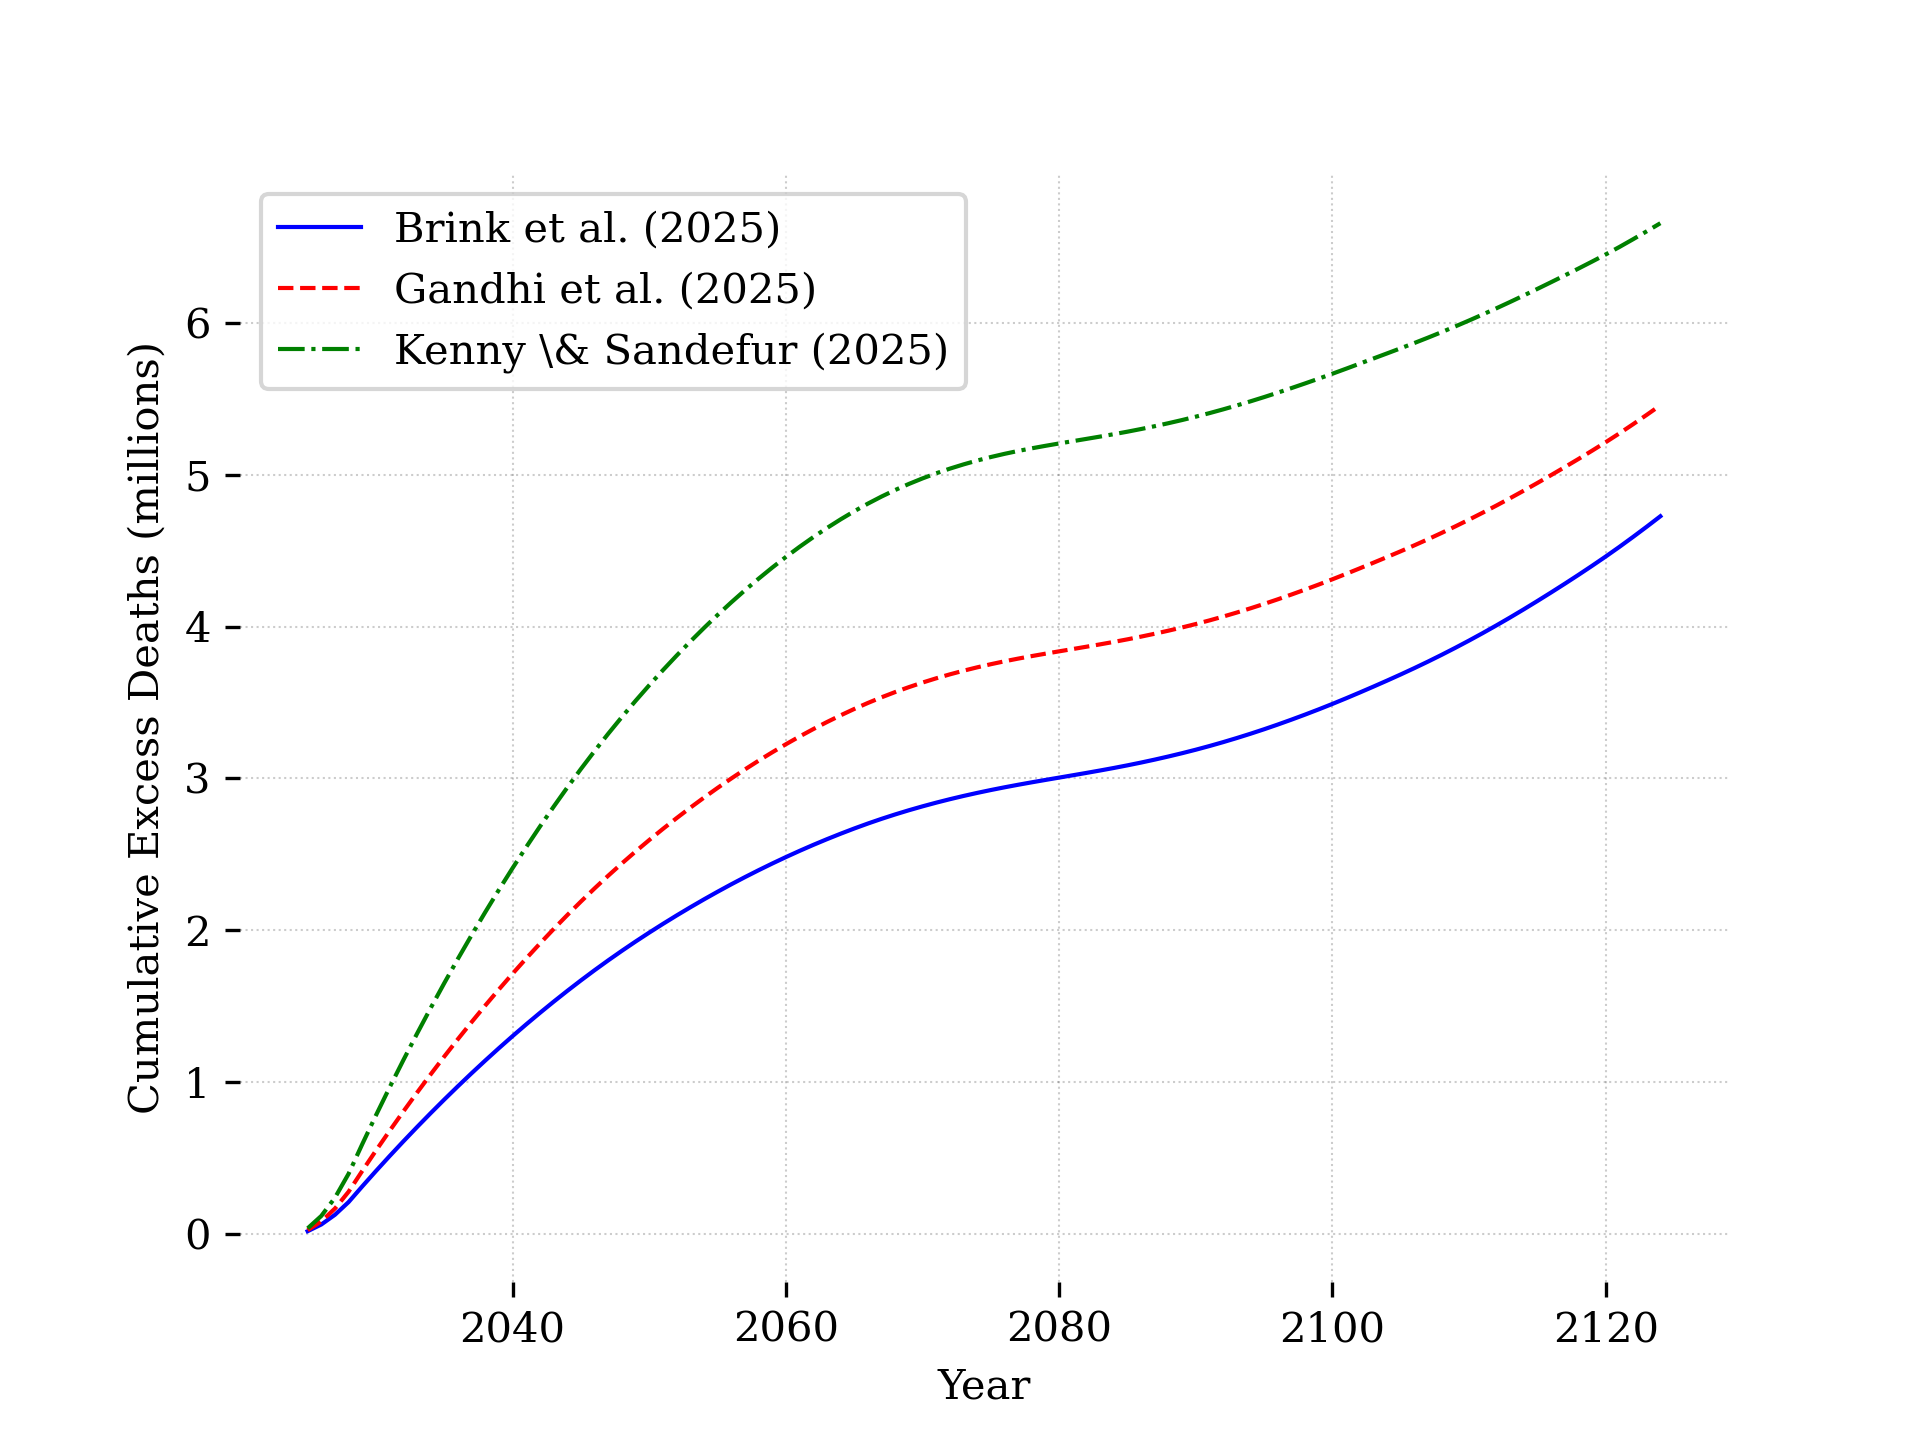
\includegraphics[scale=0.75]{./tables_figures/cumulative_excess_deaths.png}
\end{figure}

These estimates of excess deaths a mapped into the model through changes in the age-specific mortality rates.  Specifically, we begin with current age specific mortality rates as reported by the United Nations World Population Prospects 2024 \citep{UN2024}. We then apply a percentage adjustment to the mortality rates at each age to match the forecasts of excess death under each scenario. Figure \ref{fig:Mortality} shows the mortality rates for each age group in 2025 under the \textit{median excess deaths} scenario. The blue line shows the mortality rates as forecast before the U.S. withdrawl of aid.  The green line represents the \textit{median excess deaths} scenario, while the red and light blue lines shows the mortality rates under the low and high estimates of excess deaths.


\begin{figure}[H]
    \caption{Mortality rates with and without aid}
    \label{fig:Mortality}
    \centering
    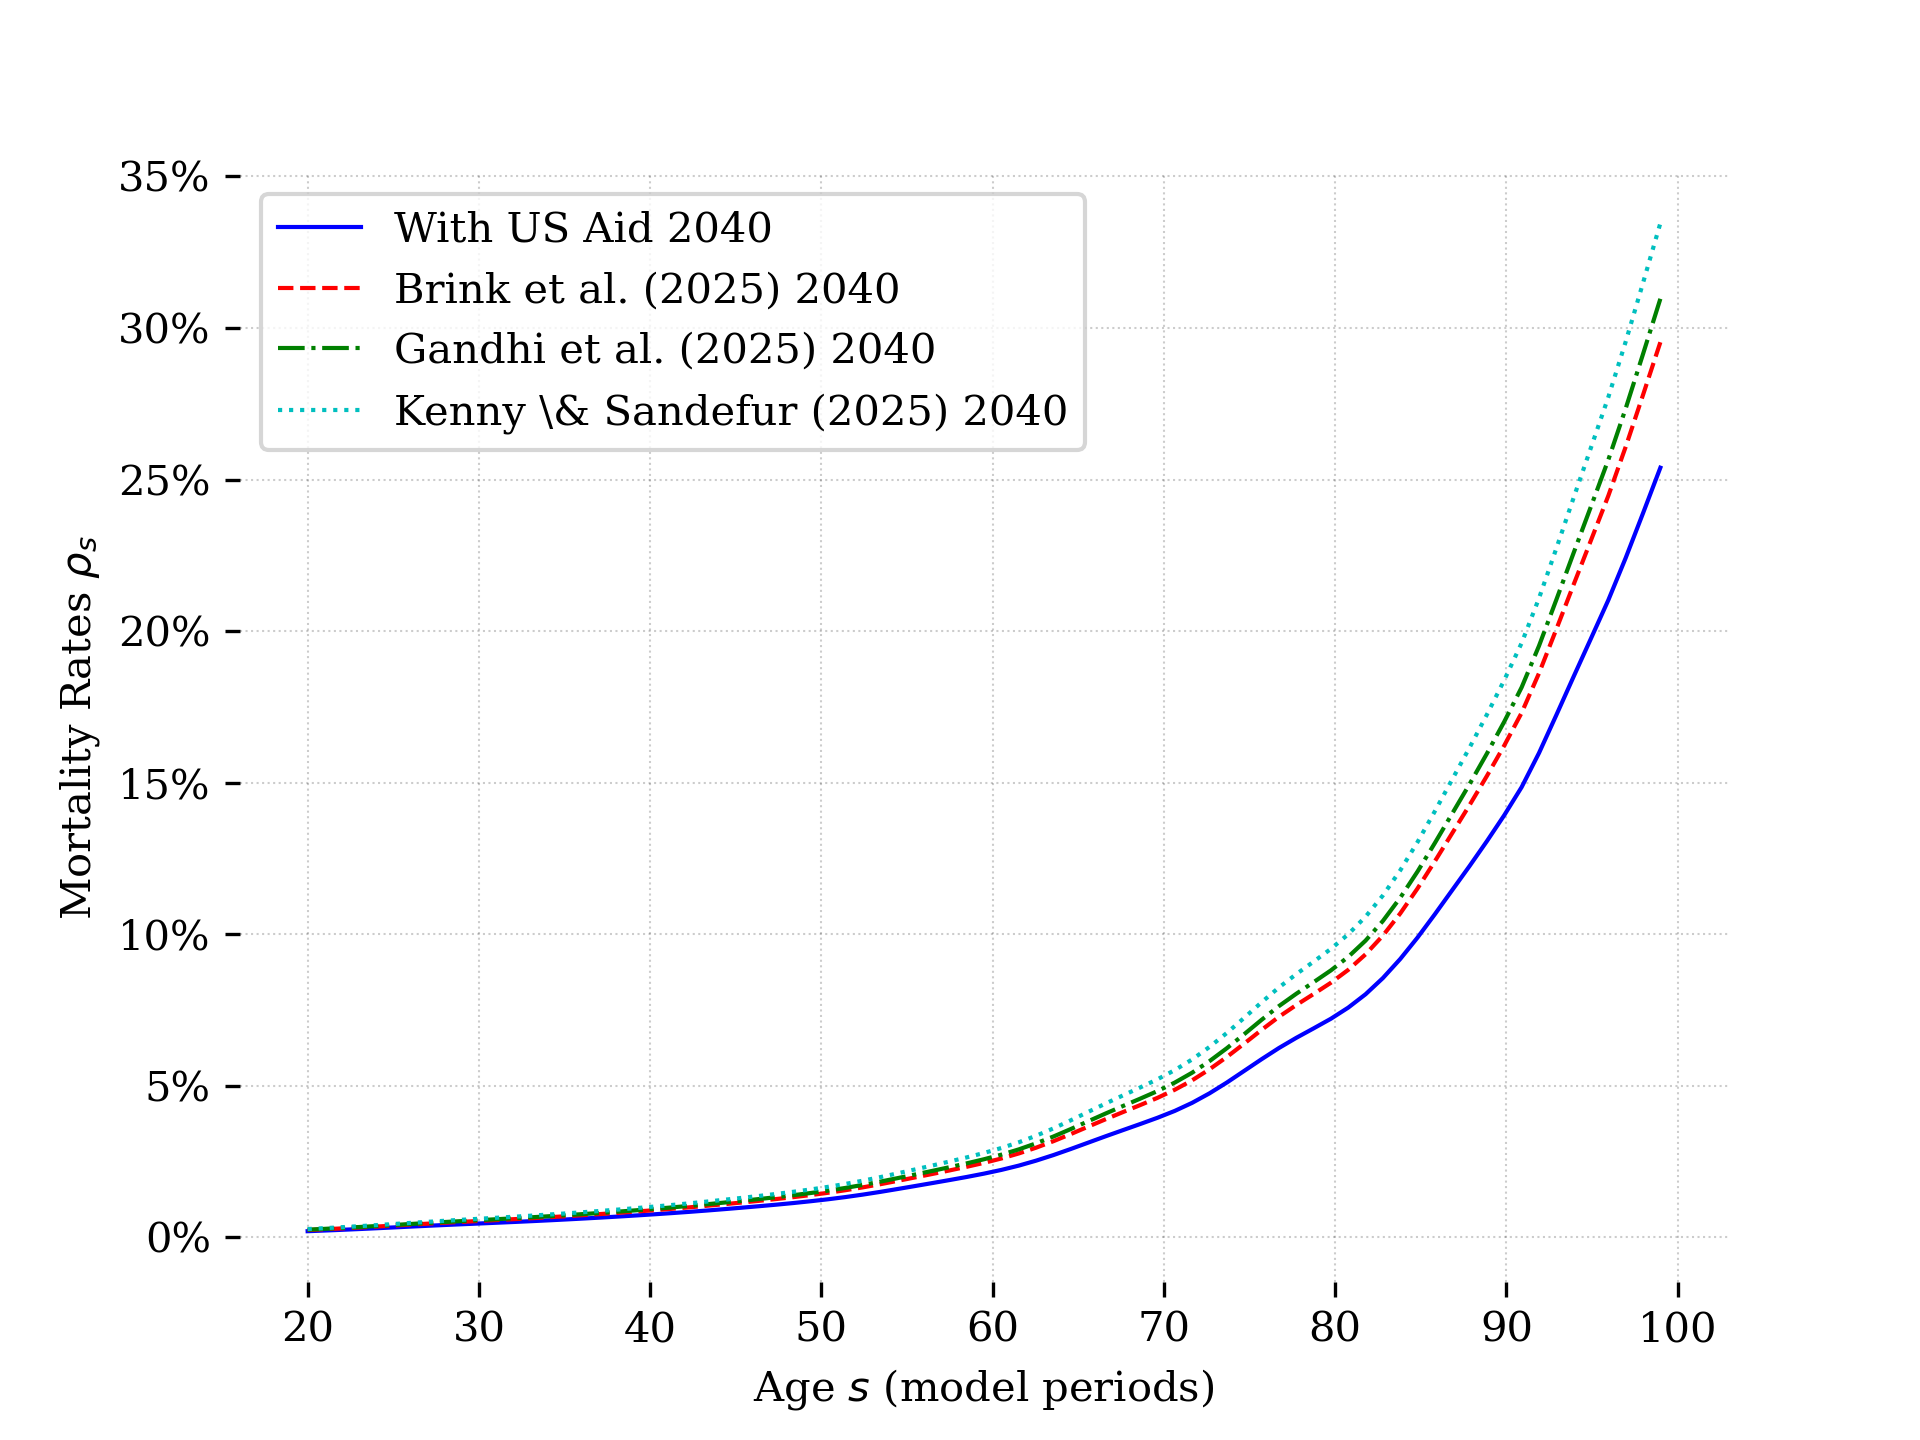
\includegraphics[scale=0.75]{./tables_figures/mortality_rates.png}
\end{figure}


% The population distribution is affected by the changes in mortality rates:
% \begin{figure}[H]
%     \caption{The population distribution with and without aid}
%     \centering
%     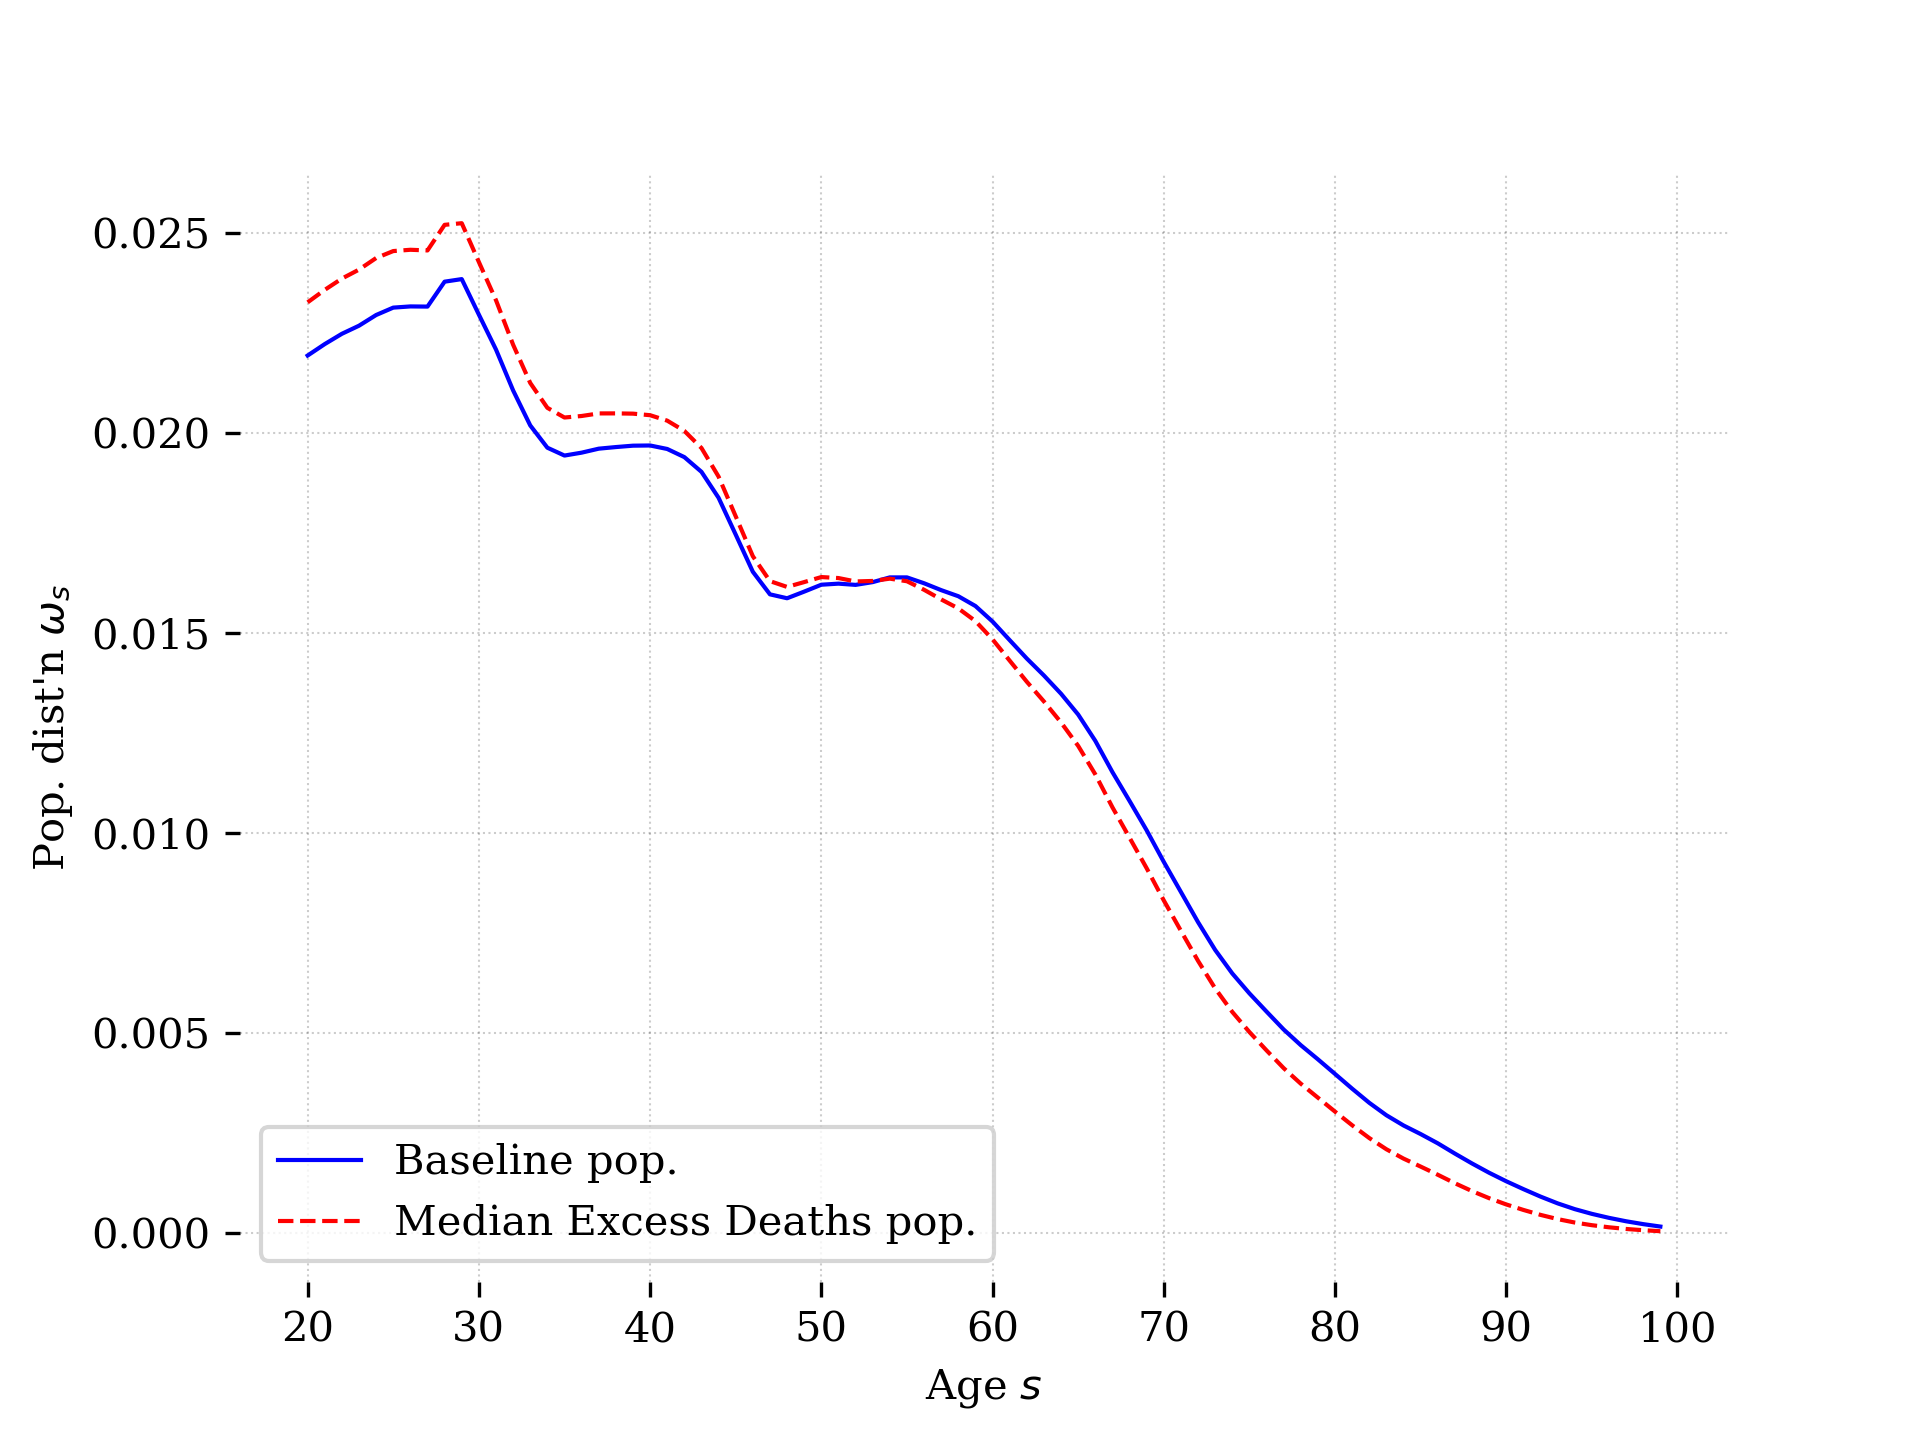
\includegraphics[scale=0.75]{./tables_figures/pop_dist_2050.png}
% \end{figure}



\subsection{Absenteeism and labor force participation}
To simulate the economic impact of disease-related morbidity among working-age individuals we impose an adjustment that reflect the effects on worker availability and productivity. This is a key margin of economic vulnerability in the absence of continued treatment and labor market support for people affected with HIV and tuberculosis.

The HIV-related productivity shock is grounded in the ILO's global estimates of the economic impact of AIDS \citep{ILO2018}. That methodology distinguishes between several channels through which HIV affects the labor market: (1) premature mortality, (2) reduced productivity among HIV-positive individuals who remain employed, (3) absenteeism due to illness or caregiving responsibilities, and (4) turnover and retraining costs. The first channel is captured using our mortality scenarios described above, while this section focuses on the productivity losses due to absenteeism and partial labor force withdrawal.

Our simulation assumes a reversal of the substantial labor market gains achieved since 2005 due to reduced HIV service coverage (e.g., PEPFAR withdrawal). ILO data for South Africa from 2005 to 2020 show a sharp decline in the number of individuals partially or fully unable to work due to HIV—from over 163,000 in 2005 to fewer than 2,300 in 2020—due to improved access to ART and labor market inclusion. To quantify this we follow the ILO's ``high impact'' scenario, which assumes that 50\% of HIV-positive individuals in the labor force become partially unable to work, and historical shares of those fully unable to work. Using 2020 ILO data, we apply this 50\% impairment rate to the estimated HIV prevalence in the labor force (23.9\%), covering adults aged 15–64. This calculation yields an effective reduction in labor productivity of 0.00361 by 2040.

For tuberculosis, we apply an additional uniform productivity penalty of 0.0002758, based on South Africa's 2023 TB incidence by age and empirical estimates of lost workdays taken from a study of the impact of tuberculosis on productivity in India \citep{Keogh2024}. The estimate assumes a high-impact scenario of 0.1442\% absenteeism loss per TB case, reflecting reduced access to diagnosis and treatment. This is applied to the prevalence of TB in the working age population and held constant over time.

The HIV-related and TB-related productivity shocks are combined to total a penalty of 0.00388 each year. This factor adjusts the labor disutility parameter in the model and is applied to the bottom 70\% of ability types among working-age individuals (ages 20–64) in the reform policy simulation.\footnote{This is the $\chi^n_s$ described in the OG-Core model documentation and reflects the relative value of leisure versus consumption in the household's utility function.} The changes are held constant throughout the simulation to reflect persistent productivity losses in the absence of expanded care.  The changes in the disutility of labor result in declines in labor force participation as we expect from increased disease prevalence.

We apply the 0.00388 adjustment in our \textit{median excess deaths} scenario, while the \textit{low excess deaths} and \textit{high excess deaths} scenarios apply 0.00194 and 0.00582, respectively.

% \begin{figure}[H]
%     \caption{Disutility of labor with and without aid}
%     \centering
%     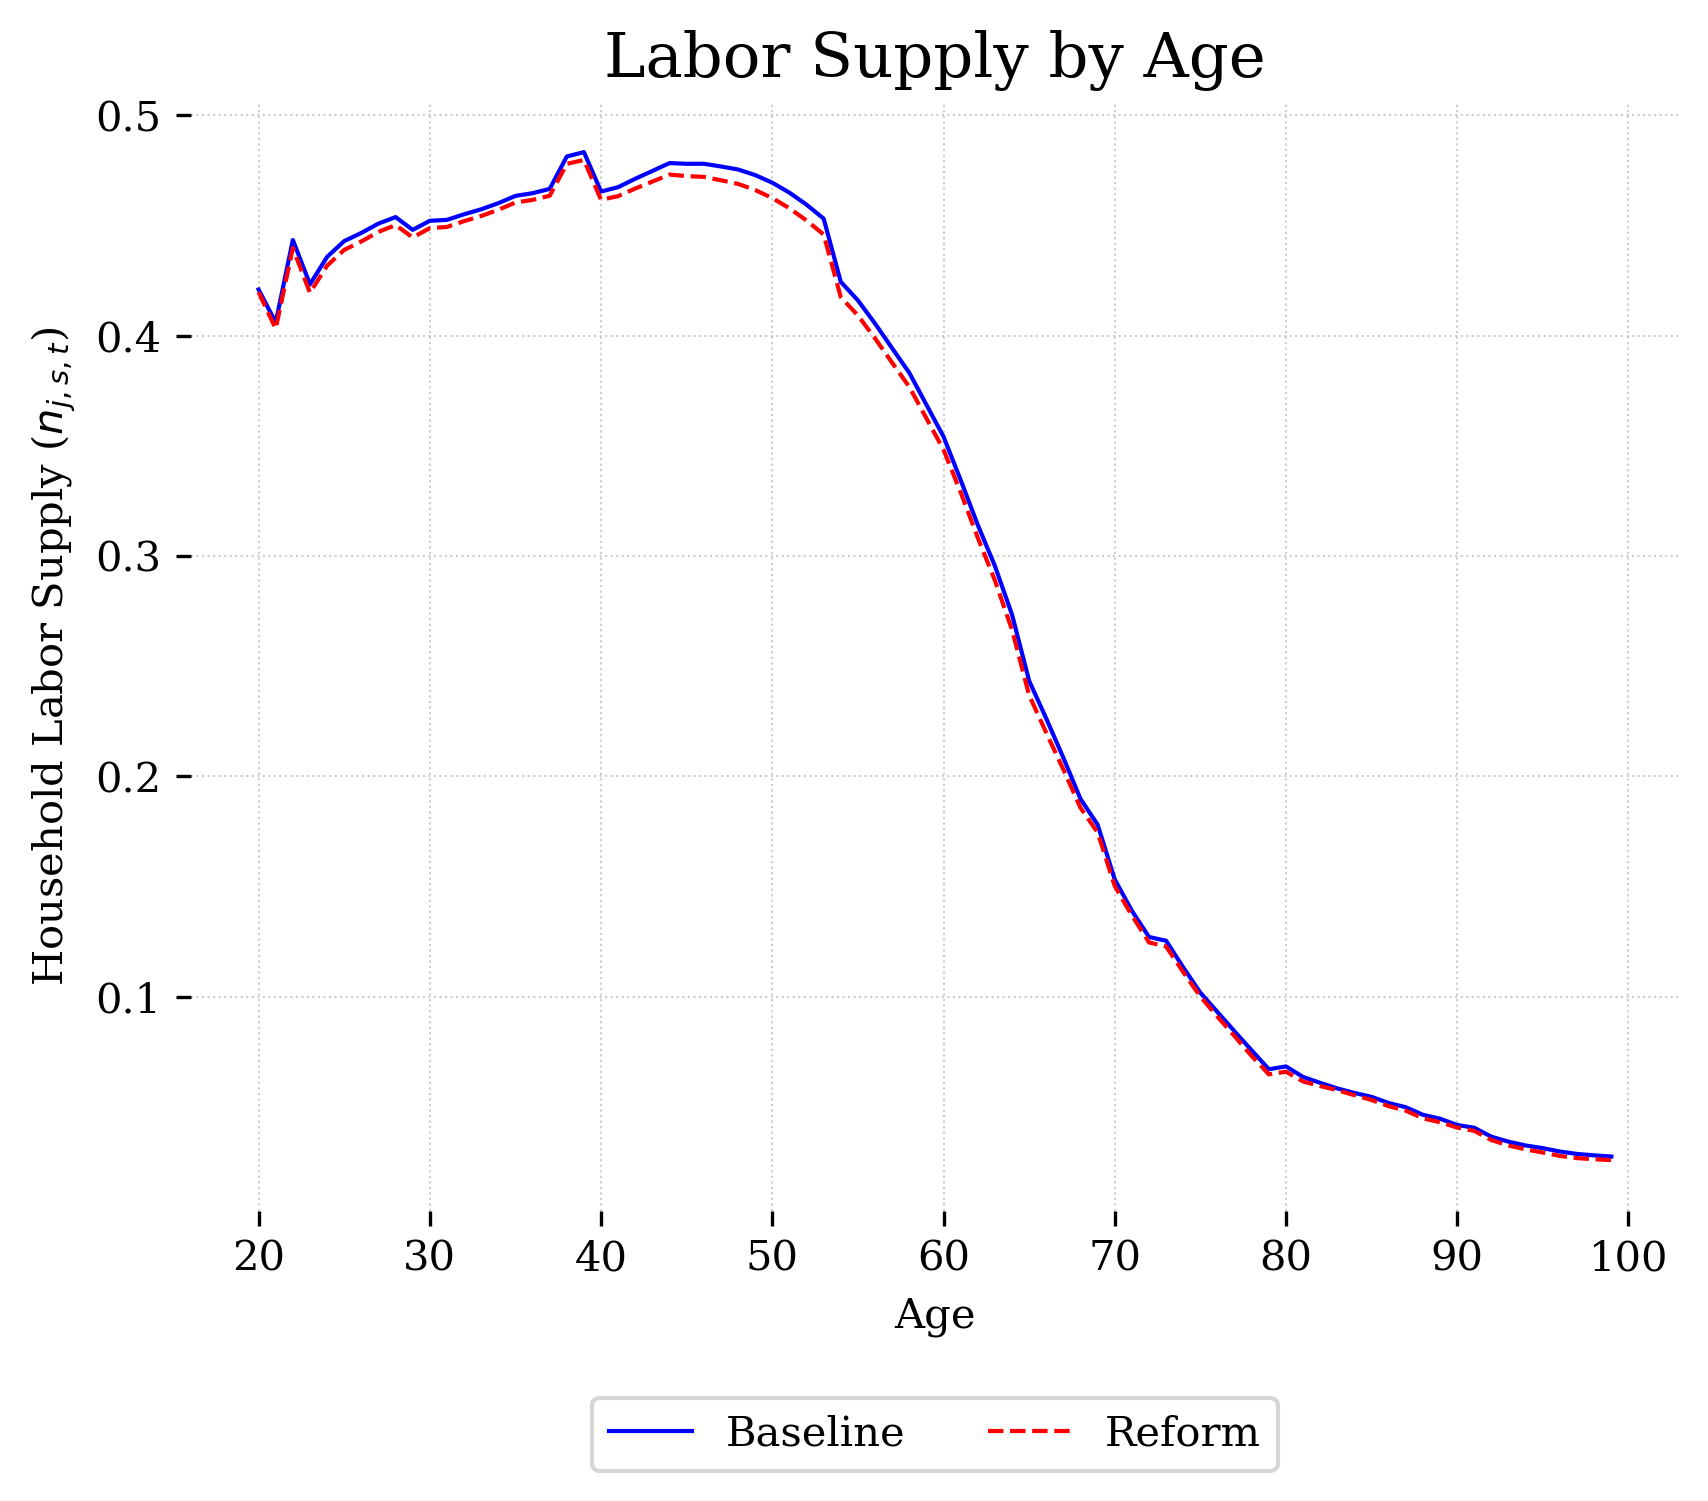
\includegraphics[scale=0.75]{./tables_figures/labor_supply.png}
% \end{figure}



\section{The Economic Costs of Disease}\label{SecResults}

We simulate each of the three scenarious described above with the aforementioned adjustments to mortality and household disutlity of work.  The simulation results show that the macroeconomic costs of a resurgence of disease in South Africa are substantial and persistent. These costs arise from sustained increases in mortality and reductions in labor force participation following the abrupt cessation of external health funding.

Table~\ref{tab:avgGDPChange} presents the average annual GDP losses over the first 20 years of the simulation horizon. In the \textit{median excess deaths} scenario—our preferred specification—South Africa's GDP declines by approximately \$21.3 billion per year (in 2025 USD). Under the \textit{low excess deaths} scenario, the annual loss is about \$11.2 billion, while in the \textit{high excess deaths} scenario, the average annual GDP loss exceeds \$31.6 billion. These losses reflect persistent reductions in effective labor supply and human capital accumulation.  Recall that \textbf{global} U.S. development assistance for health as about \$21 billion in 2021, slightly less than the average annual GDP loss in the \textit{median excess deaths} scenario.  And it must be noted that GDP impacts of disease are a very narrow measure of their true benefits to society.  But even with this strict metric, the costs-benefit ratio favors the side of continued support for health systems in South Africa.

\begin{table}[H]
\centering
\caption{Average Annual GDP Change over 20 Years (billions of 2025 USD)}
\begin{tabular}{lr}
\toprule
 & $\Delta$ GDP, Trillions \\
\midrule
Low Excess Deaths & -0.01 \\
Median Excess Deaths & -0.02 \\
High Excess Deaths & -0.02 \\
\bottomrule
\end{tabular}

\label{tab:avgGDPChange}
\end{table}

Table~\ref{tab:NPVLosses} summarizes the net present value (NPV) of cumulative GDP losses under each scenario. In the median scenario, using a 2\% discount rate, the total discounted loss amounts to over \$3 trillion (in 2025 USD). The low scenario yields an NPV loss of \$601 billion, while the high scenario projects losses exceeding \$5.5 trillion. These values highlight the long-run macroeconomic consequences of disruptions to disease control and treatment services.  To compare these economics costs to the cost of prevention, we can take the amount of foreign assistance for health programs in South Africa before 2025 and assume this support would continue indefinitely. This assistance totaled about \$500 million per year.\footnote{Source: https://foreignassistance.gov} The NPV (at a 2\% discount rate) of this level of funding is \$25 billion.  So as a direct comparison, that the NPV of the economic costs of disease (\$3.1 trillion) is 120 times larger than the cost of prevention (\$25 billion).

\begin{table}[H]
\centering
\caption{Net Present Value of GDP Loss (billions of 2025 USD)}
\begin{tabular}{rlrrr}
\toprule
index & Discount Rate & Low Excess Deaths & Median Excess Deaths & High Excess Deaths \\
\midrule
0 & 2\% & -0.42 & -2.27 & -3.99 \\
1 & 4\% & -0.30 & -0.91 & -1.49 \\
2 & 6\% & -0.19 & -0.45 & -0.71 \\
\bottomrule
\end{tabular}

\label{tab:NPVLosses}
\end{table}

These results indicate that the economic burden of disease extends far beyond the direct costs to the health sector. Even in the more optimistic scenario, where the health system absorbs much of the shock, the loss in output is substantial. The high-impact scenario shows that a collapse in treatment access and mitigation capacity could result in GDP losses equivalent to 7.5\% of South Africa's GDP.



\section{Conclusion}\label{SecConc}


This analysis shows that the economic costs of a resurgence in disease following the abrupt withdrawal of external health aid are both large and persistent. In South Africa, the median scenario—grounded in epidemiological projections and labor market data—suggests net present value GDP losses of over \$3.1 trillion USD. Even in the most optimistic case, estimated losses exceed \$600 billion in net present value. In the high-impact scenario, losses top \$5.5 trillion, over 220 times the amount of pre-2025 U.S. health assistance to South Africa. Thus, losses are not only large in absolute terms; they are disproportionate relative to the funding at stake.

The economic damage stems not only from increased mortality, but also from more subtle and compounding effects: labor market withdrawal and reduced productivity. These channels reinforce each other over time, undermining growth and worsening inequality. While the health consequences of aid withdrawal are immediate and visible, the economic consequences unfold more slowly—and are therefore at risk of being underestimated.

Our results underscore the fragility of growth in settings of high disease burden and where treatment access hinges on foreign aid. They also highlight the risks of short-term budget decisions with long-term developmental consequences. Sustaining global health investments is not only a moral imperative but also a sound macroeconomic strategy.


\end{spacing}

\section*{Data availability}

All Python code and documentation for the computational examples and analyses are available at \href{https://github.com/OpenSourceEcon/CostOfDisease}{https://github.com/OpenSourceEcon/CostOfDisease}.
\bibliography{disease.bib}


\end{document}